%=======================================================
\section{Bridging the Physical and Digital Space}
%=======================================================



\section{Engineering \acl{DT} Interoperability}
\label{sec:engineering-interoperability}

Figure \ref{fig:dt_application_example} represents a \ac{DT} implemented following the abstract architecture presented in Section \ref{sec:dt_modeling} in an exemplary deployment setting.
It highlights the role of the \ac{DT} as a bridge between \emph{physical} devices and \emph{digital} applications.
% By abstracting the complexity of connecting with the \ac{PT}, the \ac{DT} provides a digital replica tailored to application-specific requirements.

At an appropriate abstraction level, a \ac{PT} may be digitalized by obtaining and sending data through possibly \emph{several} different \texttt{Communication Channels}, which 
encompass network protocols, data formats, and physical connections.
The \ac{PI} manages interactions with the \ac{PT}, integrating such channels.
%
Similarly, on the digital side, the \ac{DT} supplies data and insights to applications via the \ac{DI}, adapting to different protocols and representations.

% Engineering the \ac{PI} and \ac{DI} requires addressing the challenge of effectively integrating such heterogeneous communication channels.
%
We argue that to ensure flexibility and adaptability, it is essential that the core of the \ac{DT}, including its models and implemented behaviors, remains decoupled from the heterogeneous physical and digital communication channels.% involved in interacting with \acp{PT} and applications.
%
The \ac{DT}'s shadowing process should focus solely on understanding the available physical data, receiving and transmitting telemetry information, and executing action requests, with no concern for the underlying implementation details.
%
This separation of concerns should be supported by the \ac{DT} architecture and achieved through a modular design of the \ac{DT} components, which has been proven effective~\cite{requirements-patterns-dt-industry-bellavista-2023,bellavista2024fgcs} as it strengthens extensibility, interoperability and maintainability with respect to monolithic approaches.

In the remainder of this section, we present our proposal for the design the \ac{DT}'s \ac{PI} and \ac{DI}, refining and extending the conceptual model originally proposed in \cite{web-of-dt-ricci-2022} with a concrete implementation based on the concept of modular \emph{adapters}.

\subsection{Physical Interoperability}
\label{sec:physical_interoperability}

%%%
% \begin{figure}[t]
%     \centering
%     \includegraphics[width=\columnwidth]{images/dt_interoperability_physical.pdf}
%     \caption{PI design with modular physical adapters each producing the corresponding \acl{PAD} that is processed by the \ac{DT} Model.}
%     \label{fig:physical_interoperability}
% \end{figure}


%\afterpage{%
  \begin{figure*}[h!]
    \setlength{\belowcaptionskip}{-5pt}
    \centering
    \begin{subfigure}{0.5}
        \centering
        \includegraphics[width=\linewidth]{figures/dt-interoperability/dt_interoperability_physical.pdf}
        \caption{Physical Interface}
        \label{fig:physical_interoperability}
    \end{subfigure}
    \begin{subfigure}{0.5}
        \centering
        \includegraphics[width=\linewidth]{figures/dt-interoperability/dt_interoperability_digital.pdf}
        \caption{Digital Interface}
        \label{fig:digital_interoperability}
    \end{subfigure}
    
    \caption{DT interfaces and their responsibilities to enable and support cyber-physical interoperability.}
    \label{fig:benchmark_webapp}
  \end{figure*}
%}

One of the main challenges in facilitating effective communication through the \ac{PI} is the wide variety of communication protocols and data formats used by \acp{PT}.
%
While it can be the case that one \ac{PT} is directly sending all the data concerning its digitalization through only one channel,
it is far more common to build a \ac{DT} aggregating different sources of information~\cite{qi2018dt-and-bigdata}.
%
\ac{IoT} protocols often differ considerably based on the manufacturer, device type, or application domain, making it difficult for the \ac{DT} software to integrate diverse assets.

% Regardless of the underlying complexity,
% from an engineering perspective,
% it is essential to decouple the \ac{DT} model from the communication requirements of the \ac{PT}.
%
We argue that the modularity of the \ac{PI}, which encapsulates these responsibilities, is a crucial factor in the design and implementation of interoperable \acp{DT}.
%
Hence, we propose the \ac{PI} to be designed as composed of multiple \emph{\acp{PA}}: specialized modules capable of interacting with the \ac{PT} using diverse protocols and data formats.
%
As shown in Figure \ref{fig:physical_interoperability}, each \ac{PA} is responsible for mediating the bi-directional interaction through a single communication channel, simplifying the design and reusability of the component, and making it configurable to adapt to different application contexts.
%
The responsibility of the \ac{PI} becomes then to manage the different \acp{PA} and make sure the \ac{DT} model can accurately interpret, process, and leverage the data generated by the physical world to create the digital replica and implement its behaviors.
%
Note that although we borrow the terminology of \ac{PA} from \cite{web-of-dt-ricci-2022}, where it is originally introduced, our proposal differs significantly.
The \emph{Physical Asset Adapter} proposed in \cite{web-of-dt-ricci-2022} is infact a conceptual monolithic component, whereas in our concrete proposal, we consider a \ac{PA} as a single-responsibility module of a potentially more complex \ac{PI}.

\subsubsection{Generating \aclp{PAD}}

To facilitate the process of managing different \acp{PA}, we introduce the idea of generating a \emph{\ac{PAD}}: a representation of the capabilities made available by a communication channel in terms of \emph{properties}, \emph{actions}, \emph{events} and \emph{relationships} that characterize the associated \ac{PT}.
%
Each \ac{PA}, since it encapsulates the characteristics of a channel, can generate the corresponding \ac{PAD}, effectively decoupling the asset's functionality from the specific communication protocols used.
%
The implementation of the \ac{PAD} generation can be challenging due to the varying capabilities of different communication protocols.
For instance, protocols like CoAP\cite{RFC7252} often come with built-in description and discovery functionalities, which can simplify the process of creating a \ac{PAD} by providing standardized representations of the physical asset's capabilities and behaviors.
On the other hand, protocols like MQTT may require developers to add additional information manually to define how information is structured and exchanged, as they do not natively include asset metadata \cite{mqtt}.
In the case of custom or proprietary protocols, the challenge becomes even more pronounced, as these protocols are tailored to specific systems and may lack any standardization or descriptive capabilities.

In all the aforementioned scenarios, the mechanism of \ac{PAD} generation offers a way to encode knowledge about the \ac{PT} bridging the gap by interpreting and extracting relevant information from the protocol used in the associated communication channels.
%
Confining this complexity within the \ac{PI} allows the \ac{DT} model to be agnostic with regard to the complexity of the underlying physical world.

The \ac{PAD} allows the \ac{PI} to discover, extract, and manage asset information and present it to the model that can choose which ones are relevant for the implementation of the \ac{DT} behavior.
%
For example, to create the \ac{DT} of a temperature sensors streaming binary data on MQTT, the \ac{PI} could be composed of a generic MQTT adapter, configured to correctly parse the payload as a decimal number, and generate a \ac{PAD} which advertise the available temperature property to the \ac{DT} model as a Celsius value. 

\subsubsection{\aclp{PAD} in the \ac{DT} Lifecycle}

The modular design of the \ac{PI} has an impact on the \ac{DT} lifecycle presented in Figure \ref{fig:lifecycle}.
%
Specifically, it tackles the open challenge of transitioning from the \texttt{Unbound} to the \texttt{Bound} state.
%
When a \ac{PA} successfully connects to the \ac{PT}'s channel and starts receiving data from it, it can send the generated \ac{PAD} to the \ac{DT} model.
The generation of the \ac{PAD} can be used as a synchronization step to signify that the \ac{PA} is successfully connected to the \ac{PT}.
%
The \ac{DT} model is then responsible for collecting the different \acp{PAD}, assessing whether all the relevant information to start computing the \ac{DT} state is available and, hence, moving on to the \texttt{Bound} phase.
%
This mechanism enables managing the \ac{DT} behavior consistently, even with the additional complexity of the modular \ac{PI} design.


\subsection{Digital Interoperability}
\label{sec:digital_interoperability}

%%%
% \begin{figure}[t]
%     \centering
%     \includegraphics[width=\columnwidth]{images/dt_interoperability_digital.pdf}
%     \caption{Digital Interface design with adapters and DT description, state and sync.}
%     \label{fig:digital_interoperability}
% \end{figure}
%%%

%%%


As \acp{DT} are meant to bridge between the physical and digital spaces,
interoperability is not only a matter of interfacing with heterogeneous devices, but also other digital applications.
Indeed, despite their initial conception as vertical silos, the concept of Digital Twins Ecosystems~\cite{web-of-dt-ricci-2022,kendall2021ndt} is emerging to support the the digitalization of complex scenarios through a combination of several \acp{DT}.
%
In this context, \acp{DT} can be used \emph{as-a-service}~\cite{liu2022state} by other applications implementing the business logic by spanning across different software entities.

To foster interoperability in ecosystems, \acp{DT} must then expose either a standardized general purpose \acf{DI} that can serve different applications or
-- following the same design principles adopted to address physical interoperability --
have a modular interface that can satisfy the different needs of different applications
as shown in Figure \ref{fig:digital_interoperability}.

As for \ac{PA} we borrow the terminology from \cite{web-of-dt-ricci-2022} and consider to have a \ac{DI} composed of modular \ac{DA}.
We thus refine the original abstract concept of \ac{DA} to represent a modular component of a more complex \ac{DI}.
Using the concept of \emph{\ac{DA}}, the \ac{DI} can expose the \ac{DT} state and services supporting multiple data formats and interaction patterns.
This can be beneficial for integrating it with applications and, especially, legacy systems.
The existence of legacy applications usually implies having little control over the integration requirements, making having more flexible \acp{DT} beneficial to better integrate with the application requirements.
% %
% One of the benefits of adopting a \ac{DT}-based design is their bridging role, shielding applications from the complexity of physical deployments.
% %
% As described in the previous section, \acp{DT} can decouple from the communication channels.
% %
% Hence, applications can leverage the \ac{DT} unified \ac{DI} instead of hardcoding against the possibly several communication channels of the \ac{PT}.
%
Using several \ac{DA}, a \ac{DT} could, for instance, support both request-response and publish-subscribe mechanisms to access its current and previous states, support different query languages to access the same data store, expose its current state using different representation formats, etc.
%
This would make the development of the application simpler because adding an application-specific \ac{DA} won't require intervention in the underlying physical system. 
%
Additionally, the developed application would be more robust and stable since it would depend only on the \ac{DT}, and changes to the physical configuration of the \ac{PT} (e.g., software updates, sensor replacement, network reconfigurations) would have no impact on the application software.
%
Even if the \ac{PT} were to change, (e.g., a software update on a robot changes the telemetry format) the \ac{DI} of the \ac{DT} could stay the same, as the changes would occur within the boundaries of the \ac{PI} and \ac{DT} model.
%
Through this mechanism, \acp{DT} effectively achieve their bridging role, shielding applications from the complexity of physical deployments.

\subsubsection{Describing \aclp{DI}}

A further level of interoperability is possible when allowing \acp{DT} to describe their \ac{DI}, advertising capabilities and available communication channels that applications can exploit.
%
% This is especially relevant in contexts where applications are not bound to a specific interface but can instead process machine-readable descriptions of \acp{DT} and choose to interact with specific assets.
%
A \ac{DT} could then use a \emph{\ac{DTD}}, which, similarly to the \ac{PAD}, can represent the features of the \ac{DT} to its observers.
%
The idea of exposing \acp{DTD} is somewhat present in the major platforms supporting the creation of \ac{DT} ecosystems, such as 
Microsoft's Azure Digital Twins\footnote{\url{https://azure.microsoft.com/en-us/products/digital-twins}} and Eclipse Ditto\footnote{\url{https://eclipse.dev/ditto/}} and is advocated by research works on interoperability in \ac{DT} ecosystems~\cite{etsi-dt-comm-requirements-2024,giulianelli2024models}.

The way such descriptions are implemented may differ significantly, but essentially, they should at least allow representing the \ac{DT}  features and APIs to access them.
%
Notably, differently from the \ac{PAD}, the \ac{DTD} is targeted to external consumers, hence, it should preferably adhere to standard formats and representations to be useful in practice in achieving interoperability.
%
To this end, using Linked Data principles\footnote{Original definition of the Linked Data principles: \url{https://www.w3.org/DesignIssues/LinkedData.html}} could be a possible solution to implement standard machine-readable \acp{DTD}~\cite{burattini2024models}.

% \begin{figure*}[t]
%     \setlength{\belowcaptionskip}{-13pt}
%     \centering
%     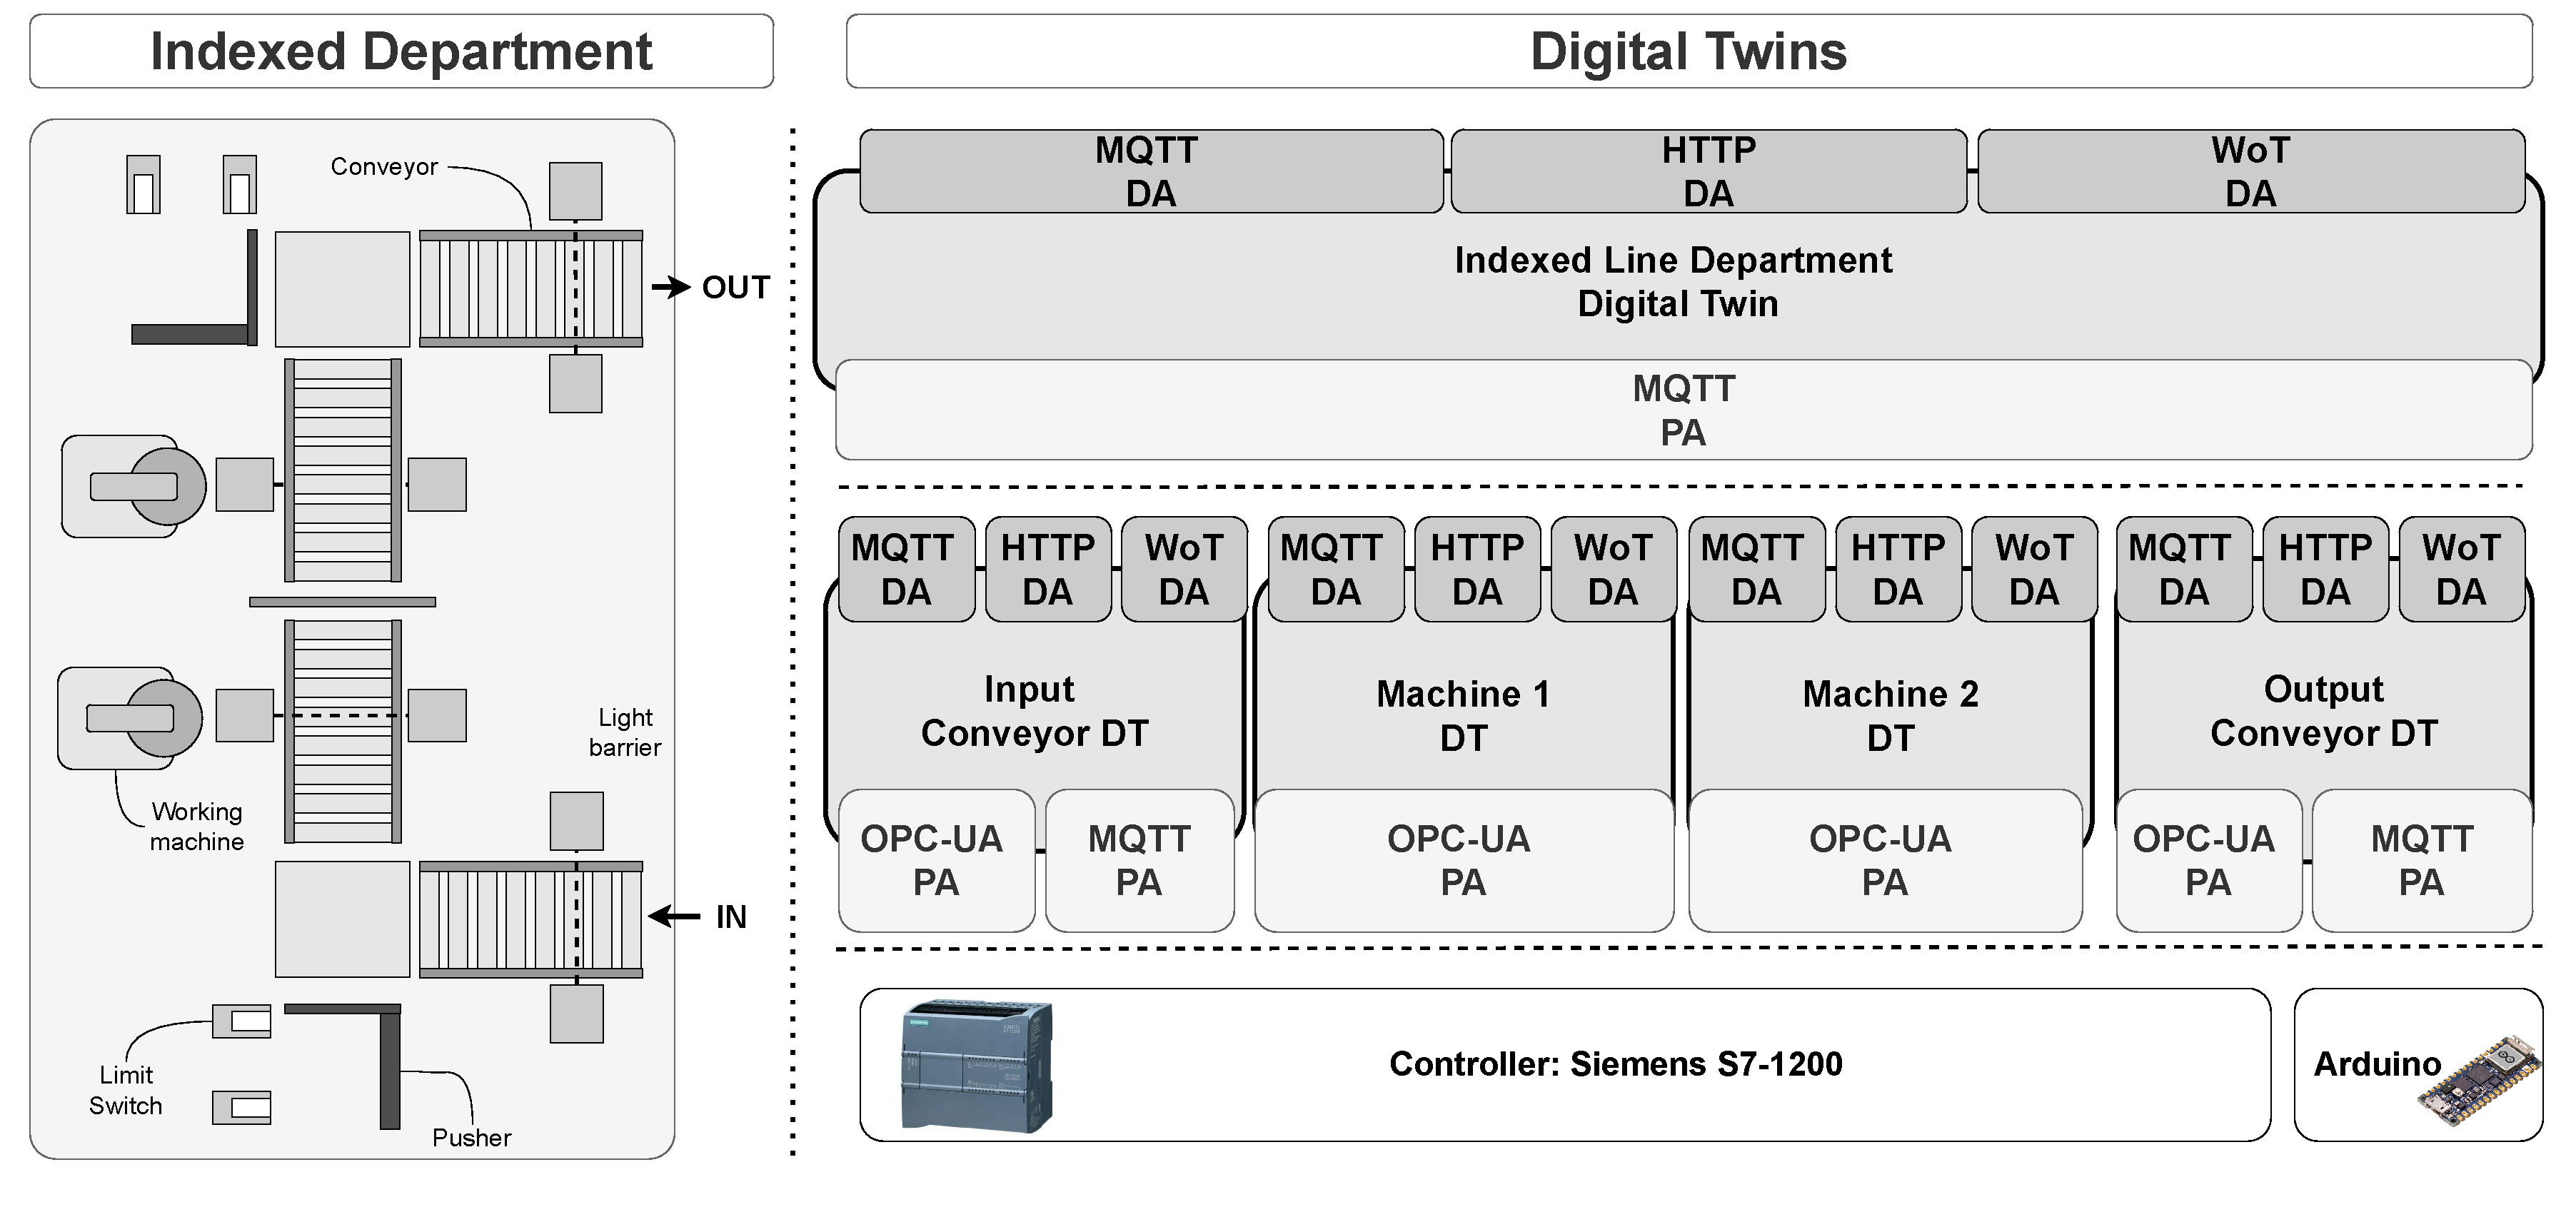
\includegraphics[width=0.93\linewidth]{figures/dt-interoperability/mf_dt_structure.pdf}
%     \caption{The \acl{DT} ecosystem architecture of the microfactory industrial system.}
%     \label{fig:mf_dt_ecosystem}
% \end{figure*}


%=======================================================
\section{Managing the Digital Twin Lifecycle}
%=======================================================

%=======================================================
\section{Modeling Augmented Behavior}
%=======================================================

%=======================================================
\section{The \acl{WLDT} Framework}
%=======================================================